\begin{center}
\begin{huge}
Διαδρομή Λαμία$\,\to\,$Αθήνα
\end{huge}
\addcontentsline{toc}{section}{Διαδρομή Λαμία$\,\to\,$Αθήνα}
\section*{Αποφυγή διοδίων Λαμίας\footnote{Λαμβάνοντας υπόψη την αναλογία ταλαιπωρίας/αξίας κομίστρου, επιλέγουμε να πληρώσουμε το κόμιστρο του συγκεκριμένου σταθμού. Στο συγκεκριμένο κομμάτι γίνονται έργα και ενδεχομένως κάποιοι δρόμοι να μην υφίστανται. Σε περίπτωση αλλαγών στο οδικό δίκτυο ή για τυχόν παραλείψεις δε φέρουμε ευθύνη.}}
\end{center}
\addcontentsline{toc}{subsection}{Αποφυγή διοδίων Λαμίας}
Ερχόμενοι από την Εθνική οδό Λαμίας - Λάρισας (Αν έρχεστε από τον Ε75 στρίψτε στον κόμβο της Αγίας Παρασκευής και συνεχίστε προς Λαμία όπου και μετά θα πάρετε την κατεύθυνση προς Αθήνα) μόλις φτάσουμε στην διασταύρωση της εικόνας (πριν από λίγο θα έχουμε περάσει ένα ΑΠ (Ανεξάρτητο Πρατήριο) στο αριστερό μας χέρι) όπου θα κάνουμε δεξιά και αμέσως αριστερά ούτως ώστε να πηγαίνουμε παράλληλα με τον Ε65.
\begin{figure}[H]
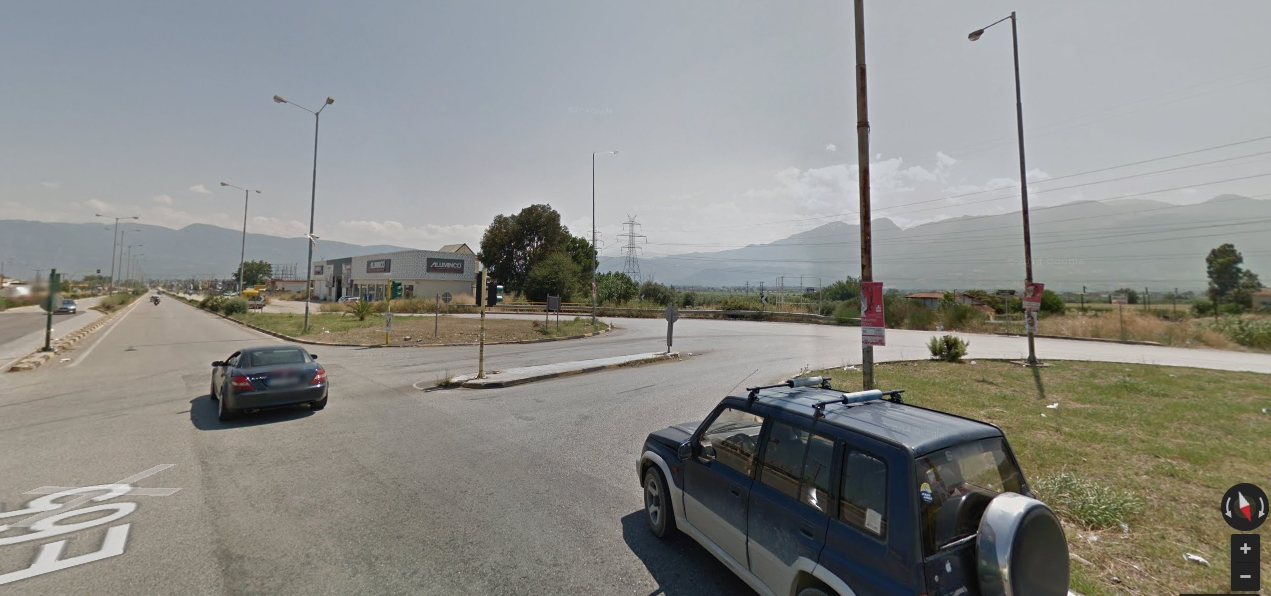
\includegraphics[width=\textwidth]{images/lamia-athina/lamia/lamia_001.jpg}
\caption{Στρίβουμε δεξιά και αμέσως αριστερά} 
\end{figure}

Συνεχίζουμε ευθεία μέχρις ότου να δούμε την Express Service στο δεξί μας χέρι. Βγαίνουμε πάλι στον Ε65 και συνεχίζουμε ευθεία μέχρι να φτάσουμε στη διχάλα της εικόνας όπου και κατευθυνόμαστε δεξιά.
 
\begin{figure}[H]
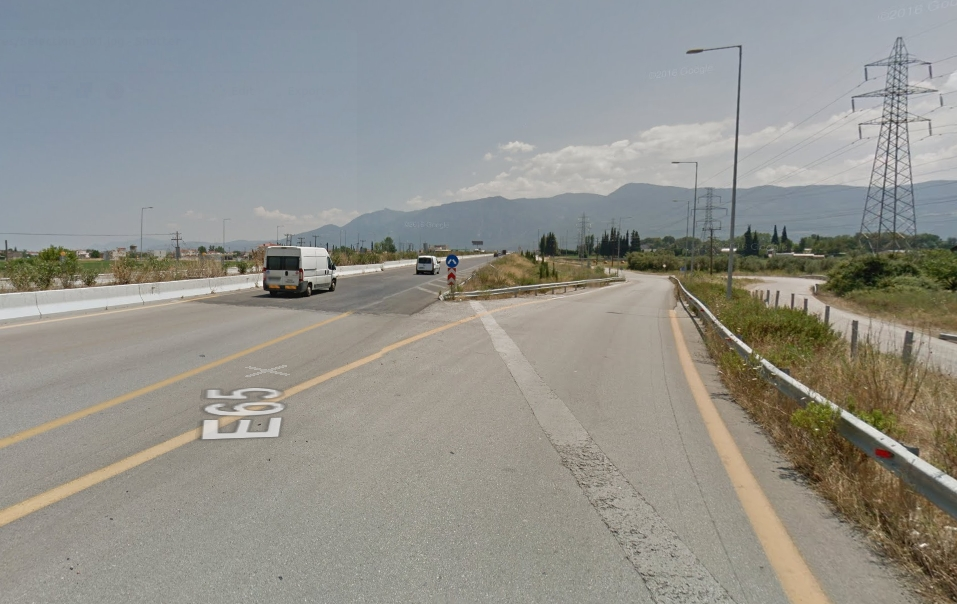
\includegraphics[width=\textwidth]{images/lamia-athina/lamia/lamia_002.jpg} 
\caption{Στρίβουμε δεξιά} 
\end{figure}

Μόλις φτάσουμε στη διασταύρωση της εικόνας (περίπου 200μ) περνάμε αριστερά και κάτω από το γεφυράκι και στη συνέχεια στρίβουμε δεξιά με κατεύθυνση προς Ανθήλη. 
\begin{figure}[H]
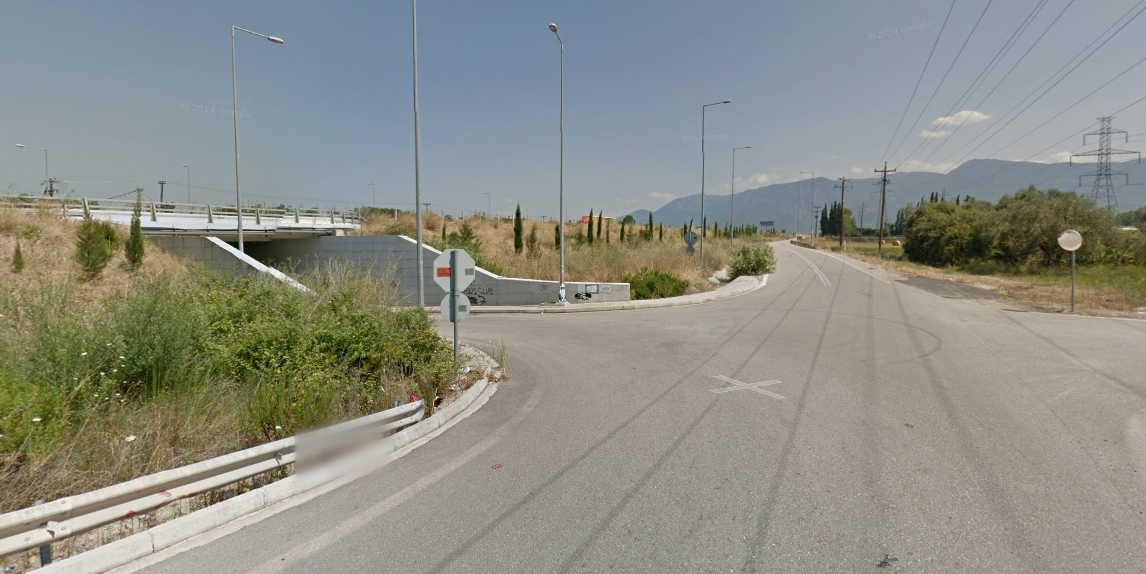
\includegraphics[width=\textwidth]{images/lamia-athina/lamia/lamia_003.jpg}
\caption{Στρίβουμε αριστερά κάτω από τη γέφυρα}
\end{figure}
\begin{figure}[H]  
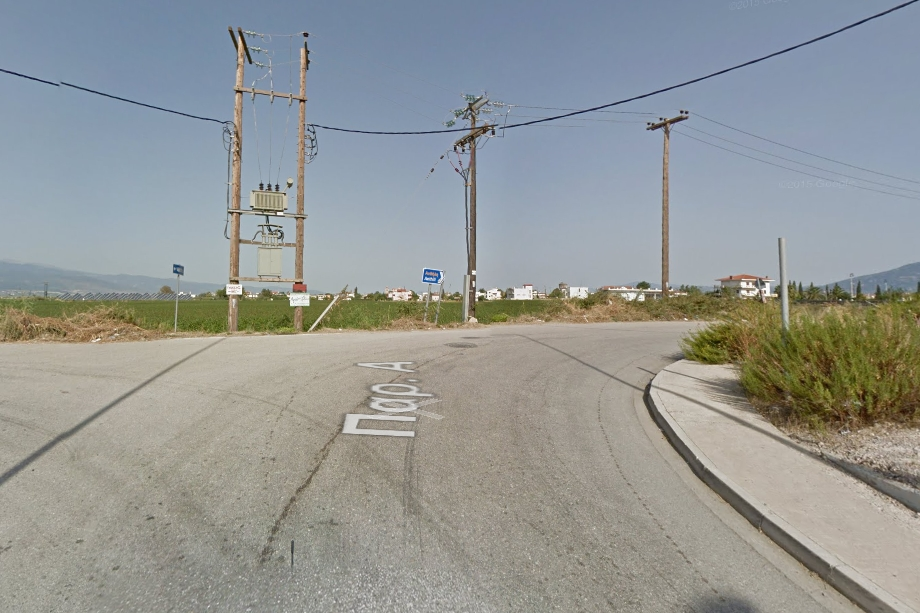
\includegraphics[width=\textwidth]{images/lamia-athina/lamia/lamia_004.jpg} 
\caption{Στρίβουμε δεξιά προς Ανθήλη} 
\end{figure}

Συνεχίζουμε για αρκετό κομμάτι του δρόμου ευθεία, περνάμε πίσω από τα Goodys και συνεχίζουμε μέχρι να φτάσουμε στο σημείο της εικόνας όπου και κάνουμε διαγώνια αριστερά. 
\begin{figure}[H]
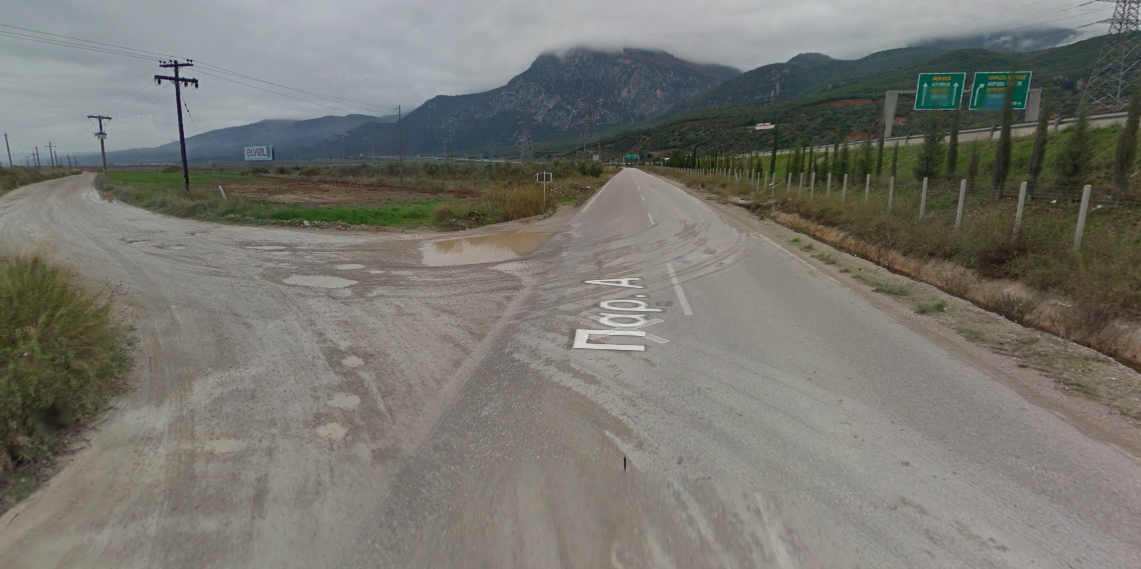
\includegraphics[width=\textwidth]{images/lamia-athina/lamia/lamia_005.jpg}
\caption{Στρίβουμε διαγώνια αριστερά} 
\end{figure}

Συνεχίζουμε με κατεύθυνση προς Θερμοπύλες. Μόλις μπούμε στις Θερμοπύλες συνεχίζουμε ευθεία κάτω από τη γέφυρα και αμέσως δεξιά και στην πρώτη έξοδο δεξιά για να μπούμε στην Επαρχιακή οδό Αταλάντης-Εξάρχου. Συνεχίζουμε ευθεία μέχρι να βρεθούμε στον κυκλικό κόμβο των Καμμένων Βούρλων και στη 2η έξοδο κατευθυνόμαστε δεξιά κάτω από τη γέφυρα και αμέσως αριστερά όπου και θα βρεθούμε στην ΠΕΟ (Παλιά Εθνική Οδό).
\begin{figure}[H]
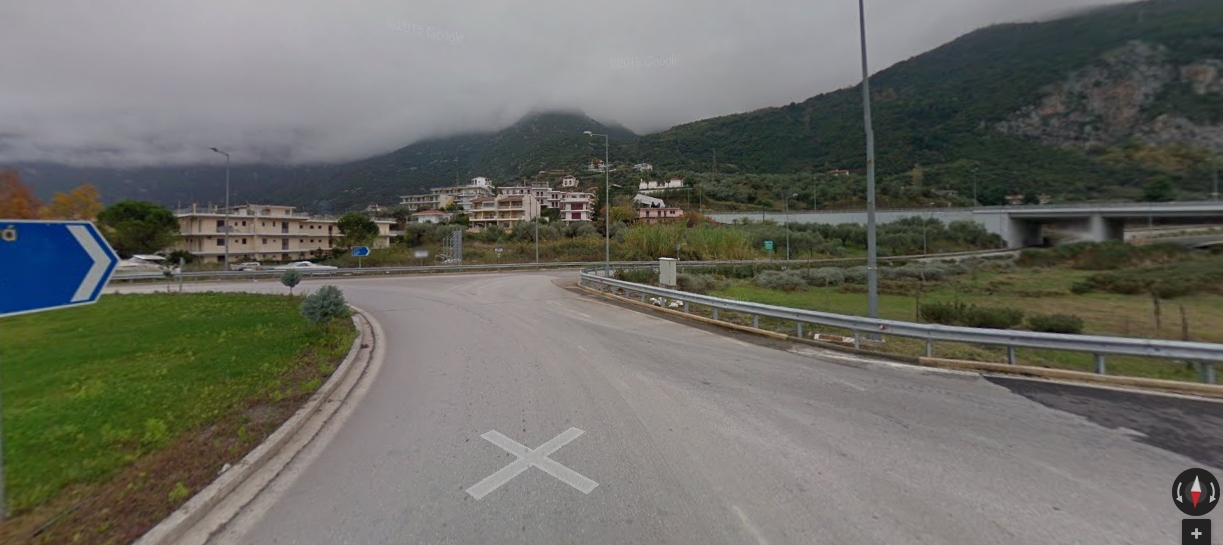
\includegraphics[width=\textwidth]{images/lamia-athina/lamia/lamia_006.jpg}
\caption{Στρίβουμε δεξιά περνάμε κάτω από τη γέφυρα και αμέσως αριστερά}  
\end{figure}

Προχωρούμε ευθεία μέχρι το σημείο της διασταύρωσης (είναι το ίδιο που χρησιμοποιούμε και για κατεύθυνση προς Λαμία) όπου κάνουμε δεξιά και προχωρούμε περνώντας κάτω από τη γέφυρα. 
\begin{figure}[H]
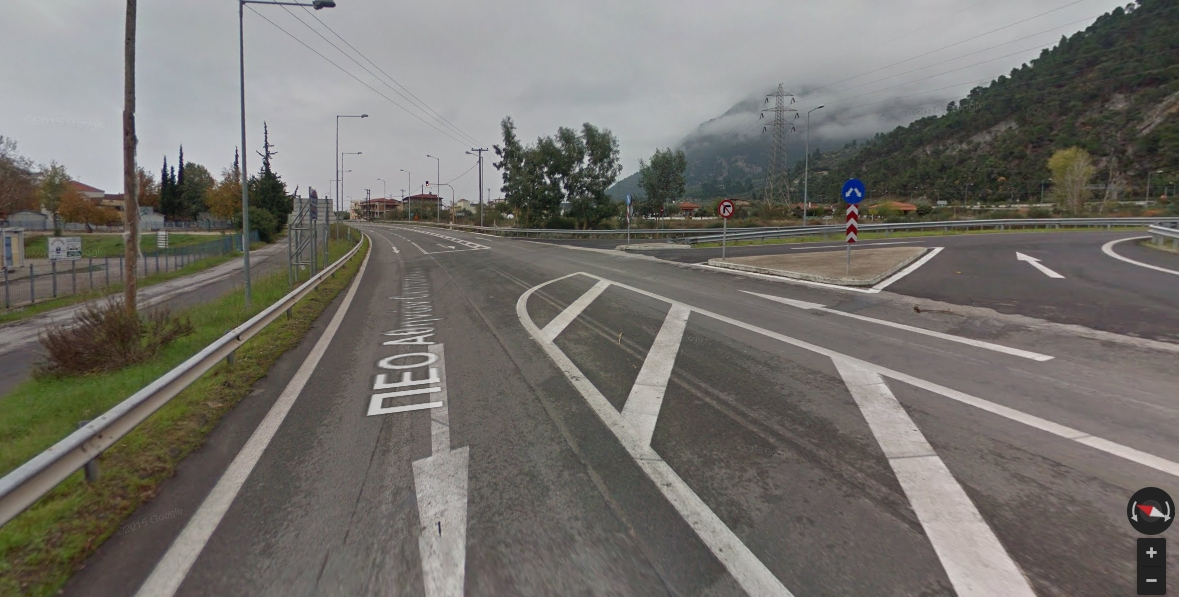
\includegraphics[width=\textwidth]{images/lamia-athina/lamia/lamia_007.jpg}
\caption{Στρίβουμε δεξιά} 
\end{figure}


Βγαίνουμε στην Εθνική Οδό.

\newpage
\begin{center}
\section*{Αποφυγή διοδίων Τραγάνας}
\end{center}
\addcontentsline{toc}{subsection}{Αποφυγή διοδίων Τραγάνας}
Βρισκόμαστε στην ΕΟ. Αναζητούμε την ταμπέλα για Δελφούς-Αταλάντη και στρίβουμε δεξιά. Στη διασταύρωση δεξιά και αμέσως αριστερά
\begin{figure}[H]
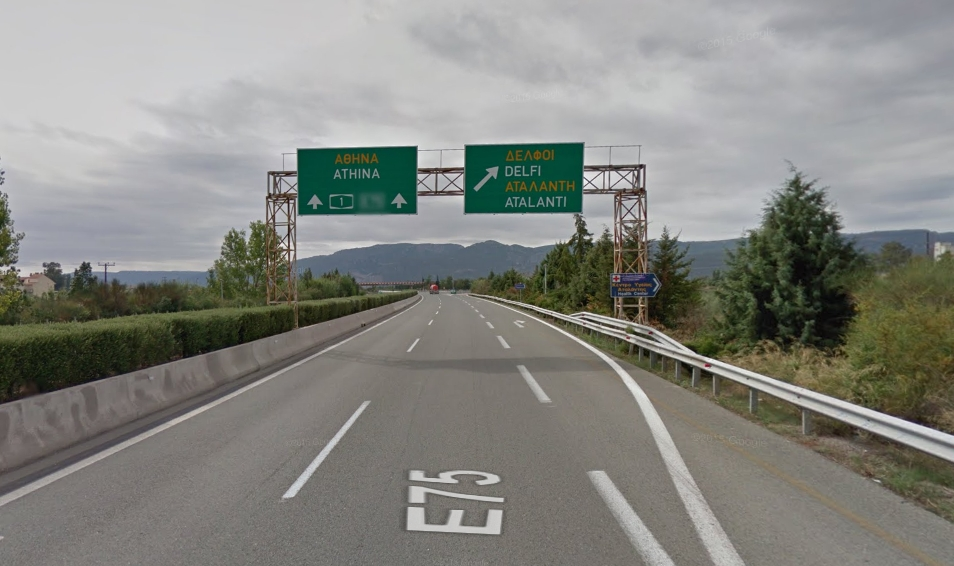
\includegraphics[width=\textwidth]{images/lamia-athina/tragana/tragana_008.jpg}
\caption{Στρίβουμε δεξιά}
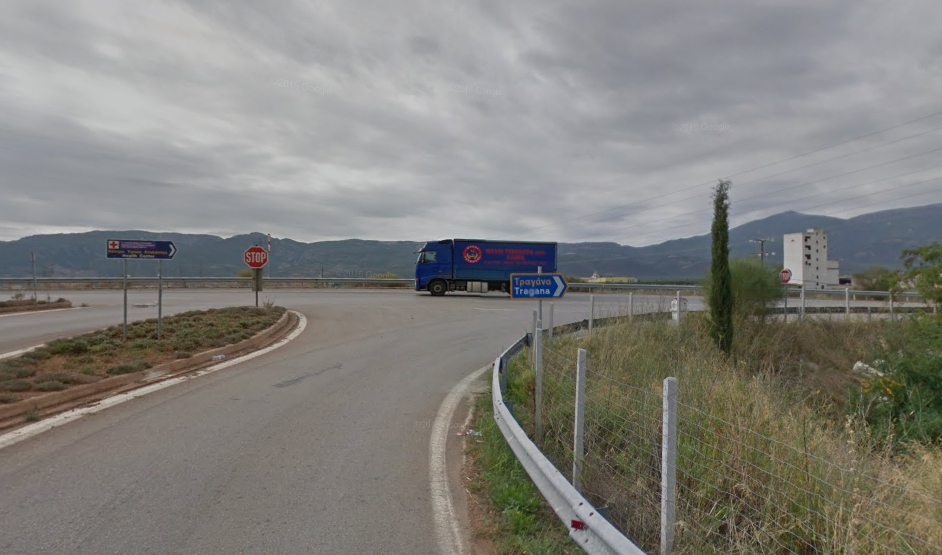
\includegraphics[width=\textwidth]{images/lamia-athina/tragana/tragana_009.jpg} 
\caption{Στρίβουμε δεξιά...}
\end{figure}
\begin{figure}[H]
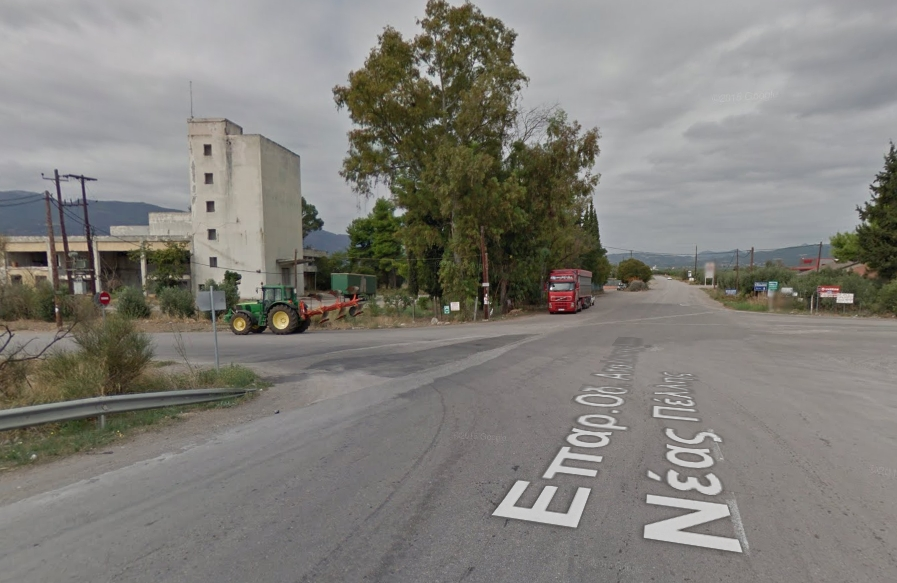
\includegraphics[width=\textwidth]{images/lamia-athina/tragana/tragana_010.jpg} 
\caption{...και αμέσως αριστερά}
\end{figure}
Συνεχίζουμε ευθεία μέχρι να περάσουμε στα αριστερά μας τα διόδια της Τραγάνας. Στο τέλος του δρόμου πηγαίνουμε δεξιά (ταμπέλα με κατεύθυνση Προσκυνά)
\begin{figure}[H]
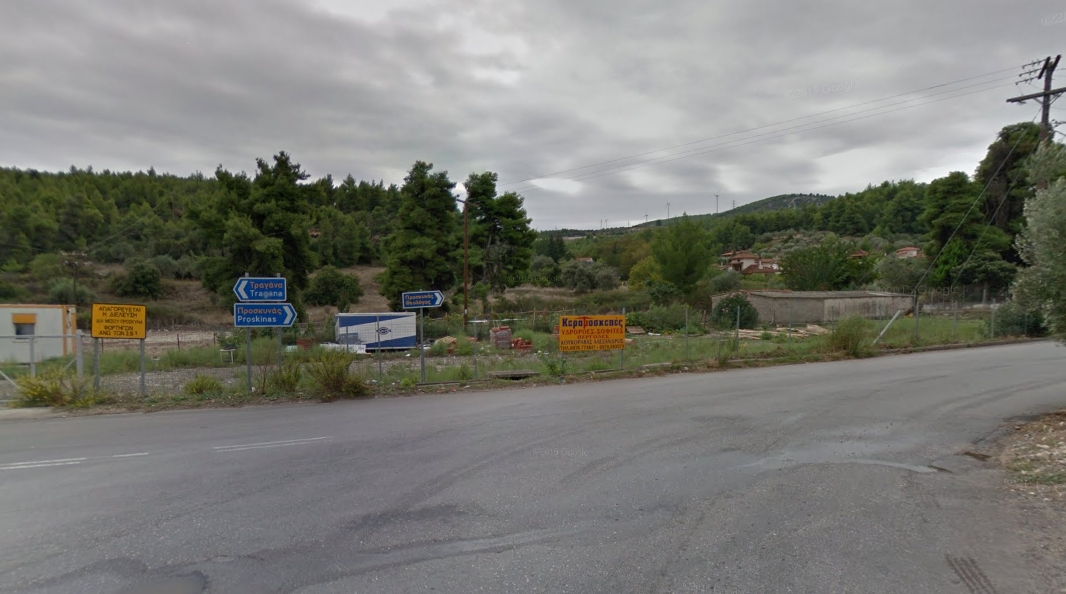
\includegraphics[width=\textwidth]{images/lamia-athina/tragana/tragana_011.jpg} 
\caption{στρίβουμε δεξιά}
\end{figure}
Μέσα στο χωριό στη διχάλα συνεχίζουμε αριστερά (Ταμπέλα προς Εθνική Οδό)
\begin{figure}[H]
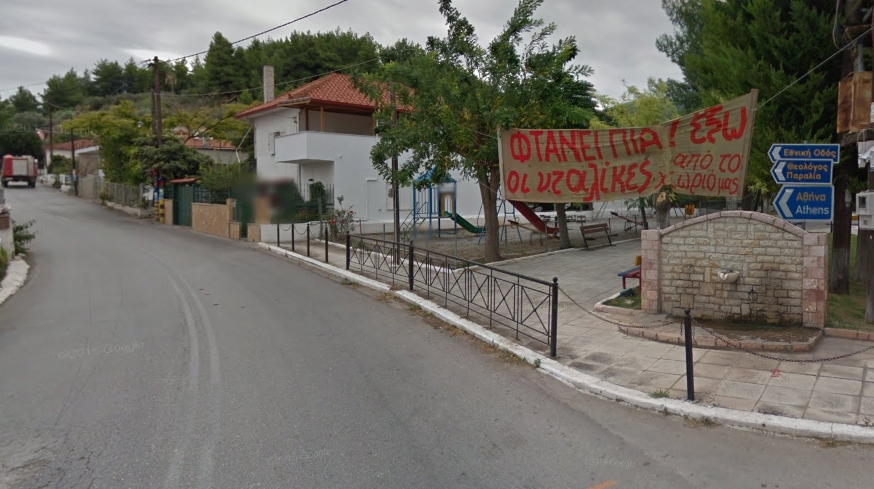
\includegraphics[width=\textwidth]{images/lamia-athina/tragana/tragana_012.jpg} 
\caption{στρίβουμε αριστερά}
\end{figure}
Συνεχίζουμε ευθεία μέχρι τη διασταύρωση όπου κάνουμε δεξιά προς ΕΟ
\begin{figure}[H]
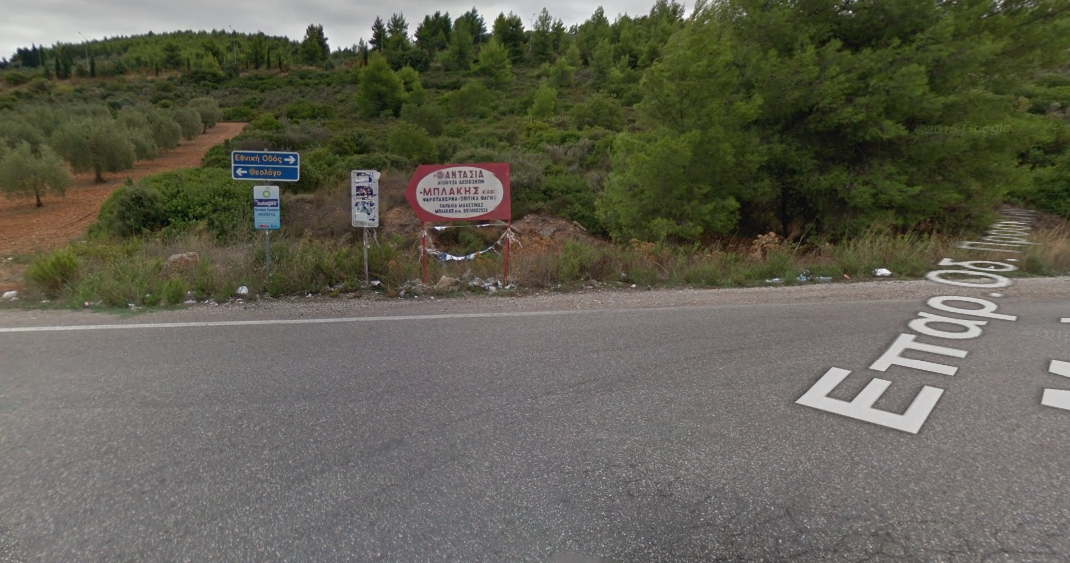
\includegraphics[width=\textwidth]{images/lamia-athina/tragana/tragana_013.jpg} 
\caption{στρίβουμε δεξιά}
\end{figure}
Τέλος φτάνουμε στη διασταύρωση που βρίσκεται αμέσως μετά το βενζινάδικο της Elin. Εκεί συνεχίζουμε ευθεία απέναντι.
\begin{figure}[H]
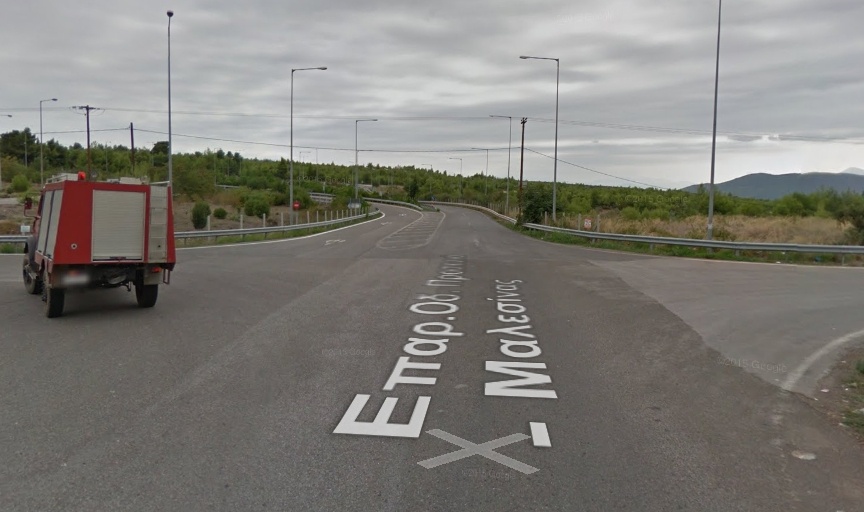
\includegraphics[width=\textwidth]{images/lamia-athina/tragana/tragana_014.jpg} 
\caption{κατευθυνόμαστε ευθεία απέναντι}
\end{figure}
Βγαίνουμε στην Εθνική Οδό.